\section{¿Ayudan las clases particulares a aprobar?}

Muchas familias recurren a las clases particulares cuando sus hijos no consiguen aprobar los exámenes. Estudiaremos si realmente son efectivas.
\begin{equation*}
    \begin{split}
        & X \equiv \text{Nota final de los alumnos que asisten a clases particulares}\\
        & Y \equiv \text{Nota final de los alumnos no que asisten a clases particulares}
    \end{split}
\end{equation*}

En nuestros datos, un $71.82\%$ de los alumnos que tomaron clases particulares aprobaron. En comparación, un $63.08\%$ de los alumnos que no fueron a clases particulares aprobaron.
\begin{equation*}
    \begin{split}
        & p_{x} = 0.7182\\
        & p_{y} = 0.6308
    \end{split}
\end{equation*}

Como en los contrastes anteriores, primero tenemos que estudiar la normalidad de la población.

\begin{figure}[H]
    \begin{center}
        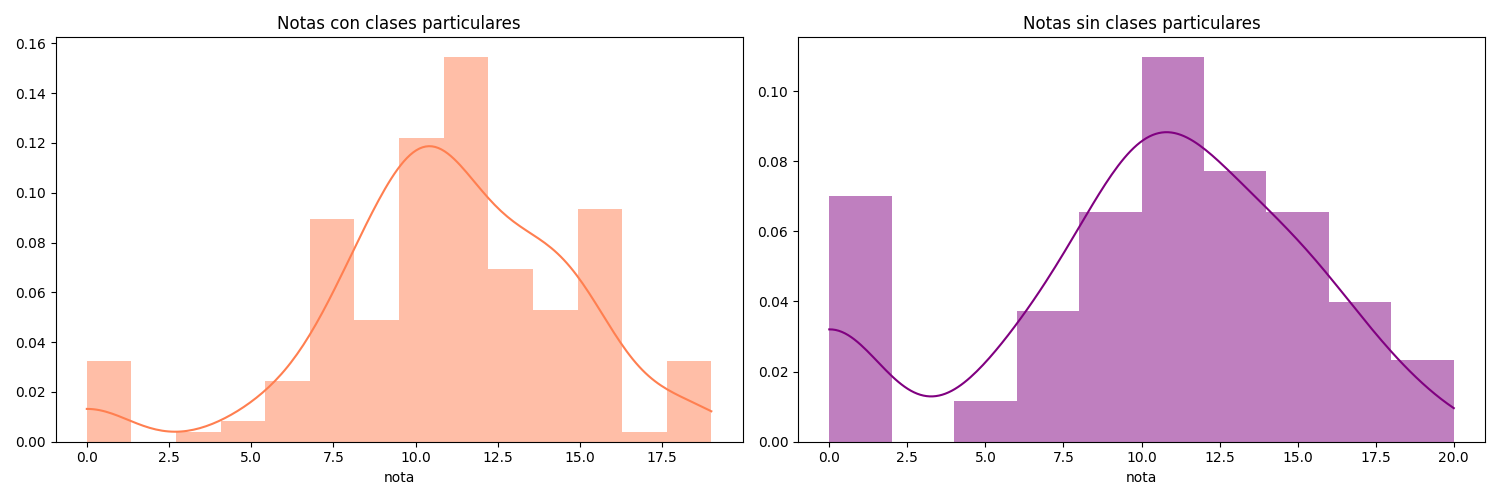
\includegraphics[width=1\textwidth]{figures/dist-notas-clases-particulares.png}
    \end{center}
    \caption{Gráficos de distribución de las notas finales de los alumnos que toman clases particulares y de los que no}
    \label{fig:dist-notas-clases-particulares}
\end{figure}

Esta vez, nos ayudaremos del QQ-plot, el cual compara los cuantiles observados con los cuantiles teóricos de la distribución normal.

\begin{figure}[H]
    \begin{center}
        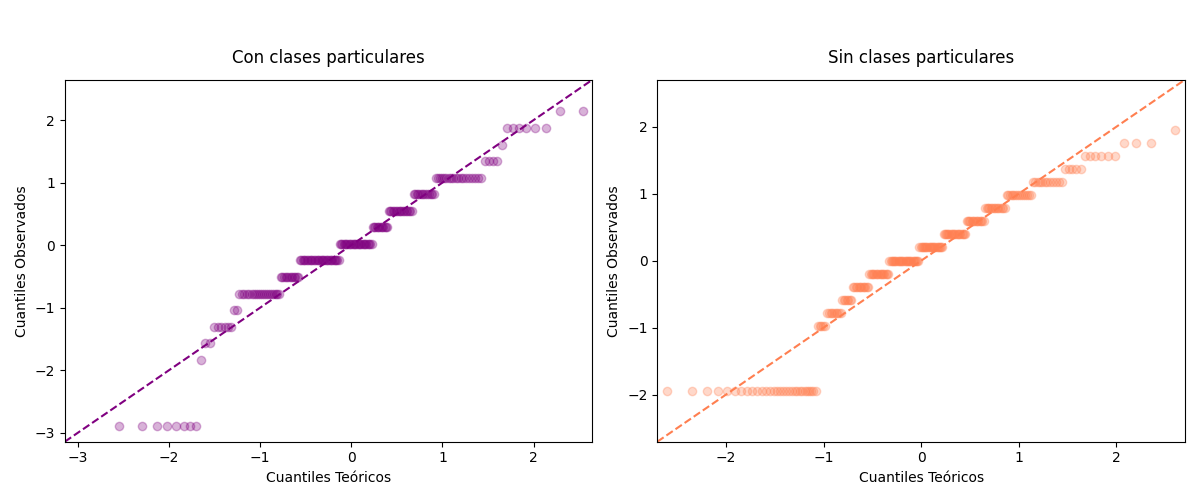
\includegraphics[width=1\textwidth]{figures/qq-plot-notas-particulares.png}
    \end{center}
    \caption{QQ-plot de las notas finales de alumnos que toman clases particulares y de los que no}\label{fig:qq-plot}
\end{figure}

Vemos que en ambos gráficos, los cuantiles se ajustan bien excepto al comienzo. Esto se debe a que hay muchos alumnos con ceros en la nota ya que no se presentaron a clase. 

Como estamos trabajando con muestras grandes y los datos presentan una asimetría moderada, utilizaremos un contraste paramétrico para la diferencia de proporciones.

\begin{equation*}
    \begin{split}
        & \gamma_{1}(x) = \frac{\sum_{i=1}^{n}(x_i - \bar{x})^3}{n \cdot s^3} = -0.70\\
        & \gamma_{1}(y) = \frac{\sum_{i=1}^{n}(y_i - \bar{y})^3}{n \cdot s^3} = -0.61
    \end{split} 
\end{equation*}

Nuestras hipótesis serán las siguientes:

\begin{itemize}
    \item \textbf{Hipótesis nula ($H_0$)}: $\pi_{x} - \pi_{y} = 0$ (no existe diferencias significativas entre las proporciones de aprobados entre los alumnos que asisten a clases particulares y de los que no)
    \item \textbf{Hipótesis alternativa ($H_a$)}: $\pi_{x} - \pi_{y} > 0$ (la proporción de aprobados de los alumnos que toman clases particulares es mayor respecto a la de los alumnos que no)
\end{itemize}

Al realizar el test obtenemos los siguientes resultados:
\begin{equation*}
    Z_{\text{obs}} = 1.8417 \Rightarrow \text{p-valor} = P(Z > 1.8417) = 0.0328
\end{equation*}

Con un $5\%$ de significación, diremos que los datos muestran evidencias suficientes como para rechazar que las proporciones de aprobados en los alumnos que toman clases particulares y de los que no no difieren significativamente. Por lo tanto, al $5\%$, aceptaremos la hipótesis alternativa de que la proporción de aprobados es mayor en los alumnos que asisten a clases particulares.
